% This is samplepaper.tex, a sample chapter demonstrating the
% LLNCS macro package for Springer Computer Science proceedings;
% Version 2.21 of 2022/01/12
%
\documentclass[runningheads]{llncs}
%
\usepackage[T1]{fontenc}
% T1 fonts will be used to generate the final print and online PDFs,
% so please use T1 fonts in your manuscript whenever possible.
% Other font encondings may result in incorrect characters.
%
\usepackage{graphicx}
\usepackage{epstopdf}
% Used for displaying a sample figure. If possible, figure files should
% be included in EPS format.
%
% If you use the hyperref package, please uncomment the following two lines
% to display URLs in blue roman font according to Springer's eBook style:
%\usepackage{color}
%\renewcommand\UrlFont{\color{blue}\rmfamily}
%\urlstyle{rm}
%
\begin{document}
%
\title{Contribution Title}
%
%\titlerunning{Abbreviated paper title}
% If the paper title is too long for the running head, you can set
% an abbreviated paper title here
%
\author{David Bacas Posadas\inst{1} \and
Julian Carrión Tovar\inst{1} \and
Minerva Cebrián Marín\inst{1} \and 
Miguel Ángel Luque Gómez\inst{1} \and 
Pablo Hernández Ibáñez\inst{1}}
%
\authorrunning{F. Author et al.}
% First names are abbreviated in the running head.
% If there are more than two authors, 'et al.' is used.
%
\institute{University of Granada, Granada, Spain}
%
\maketitle              % typeset the header of the contribution
%
\begin{abstract}
The abstract should briefly summarize the contents of the paper in
150--250 words.

\keywords{First keyword  \and Second keyword \and Another keyword.}
\end{abstract}
%
%
%
\section{First Section}

\subsection{Utilidad y Ventajas (Rol: Proponente)}
La integración de la IA Generativa en sistemas distribuidos no es un simple capricho técnico, sino una necesidad imperativa para hacer que esta tecnología sea verdaderamente útil, escalable y segura en aplicaciones reales. A continuación, se detallan las principales ventajas prácticas de esta convergencia:

\begin{itemize}
    \item \textbf{Escalabilidad horizontal extrema:} Si un problema es demasiado grande, el sistema permite añadir más recursos en red para superarlo. Esto resulta evidente al observar modelos masivos como GPT-4, los cuales son tan gigantescos que no caben en la memoria de un solo dispositivo, pero pueden ejecutarse sin problema al conectar miles de tarjetas gráficas para que trabajen coordinadas como un único gran cerebro.
    
    \item \textbf{Eficiencia y optimización de recursos (PagedAttention):} Las arquitecturas modernas gestionan la memoria de forma dinámica para no desperdiciar capacidad. Podemos imaginar una situación donde nuestra universidad lanza un tutor virtual y miles de estudiantes se conectan simultáneamente en época de exámenes; gracias a esta compartición inteligente de la memoria caché, los servidores no colapsan y todos los alumnos reciben su respuesta al instante.
    
    \item \textbf{Privacidad y soberanía de datos (Aprendizaje Federado):} Es posible entrenar modelos de IA sin que la información confidencial abandone su lugar de origen. Un escenario real de gran utilidad sería el de varios hospitales andaluces colaborando para entrenar un modelo médico; en lugar de enviar historiales a una base de datos central, la IA viaja a cada centro, aprende localmente y solo comparte el conocimiento matemático resultante, manteniendo la privacidad intacta.
    
    \item \textbf{Transparencia de acceso y ubicación:} El sistema distribuye la carga de trabajo ocultando toda la complejidad subyacente al usuario. Así, un investigador puede ejecutar una petición compleja desde su portátil y la infraestructura repartirá automáticamente el esfuerzo entre decenas de servidores lejanos, dándole la cómoda ilusión de que todo el procesamiento está ocurriendo mágicamente dentro de su propia máquina.
    
    \item \textbf{Respuestas inmediatas sin latencia (Edge AI):} Al acercar el cómputo al extremo de la red, se eliminan los tiempos de espera asociados a la transmisión de datos hacia la nube. Resulta fácil comprender la importancia de esto si pensamos en un vehículo autónomo, donde enviar el vídeo de la cámara a un centro de datos lejano para decidir si debe frenar introduciría un retraso letal, problema que se resuelve procesando esa inferencia directamente en el hardware del propio coche.
    
    \item \textbf{Alta disponibilidad y tolerancia a fallos:} El diseño distribuido garantiza que los servicios críticos nunca dejen de funcionar. De este modo, si dependemos de un asistente de IA para gestionar las operaciones de una empresa y un nodo físico sufre un corte eléctrico, el balanceador de carga transfiere inmediatamente el trabajo a otro servidor activo, de forma tan rápida que el usuario final no experimenta ninguna interrupción en el servicio.
    
    \item \textbf{Desagregación estratégica de tareas:} Este enfoque permite asignar cada fase computacional al hardware que mejor sepa realizarla. Para visualizarlo, cuando un usuario pide analizar un documento muy extenso, el sistema es capaz de enviar la fase inicial de lectura intensiva a los servidores con mayor fuerza bruta, mientras que la posterior generación del texto se delega a máquinas especializadas en ancho de banda, operando en conjunto como una cadena de montaje altamente rentable.
\end{itemize}

\subsection{A Subsection Sample}
Please note that the first paragraph of a section or subsection is
not indented. The first paragraph that follows a table, figure,
equation etc. does not need an indent, either.

Subsequent paragraphs, however, are indented.

\subsubsection{Sample Heading (Third Level)} Only two levels of
headings should be numbered. Lower level headings remain unnumbered;
they are formatted as run-in headings.

\paragraph{Sample Heading (Fourth Level)}
The contribution should contain no more than four levels of
headings. Table~\ref{tab1} gives a summary of all heading levels.

\begin{table}
\caption{Table captions should be placed above the
tables.}\label{tab1}
\begin{tabular}{|l|l|l|}
\hline
Heading level &  Example & Font size and style\\
\hline
Title (centered) &  {\Large\bfseries Lecture Notes} & 14 point, bold\\
1st-level heading &  {\large\bfseries 1 Introduction} & 12 point, bold\\
2nd-level heading & {\bfseries 2.1 Printing Area} & 10 point, bold\\
3rd-level heading & {\bfseries Run-in Heading in Bold.} Text follows & 10 point, bold\\
4th-level heading & {\itshape Lowest Level Heading.} Text follows & 10 point, italic\\
\hline
\end{tabular}
\end{table}


\noindent Displayed equations are centered and set on a separate
line.
\begin{equation}
x + y = z
\end{equation}
Please try to avoid rasterized images for line-art diagrams and
schemas. Whenever possible, use vector graphics instead (see
Fig.~\ref{fig1}).

\begin{figure}
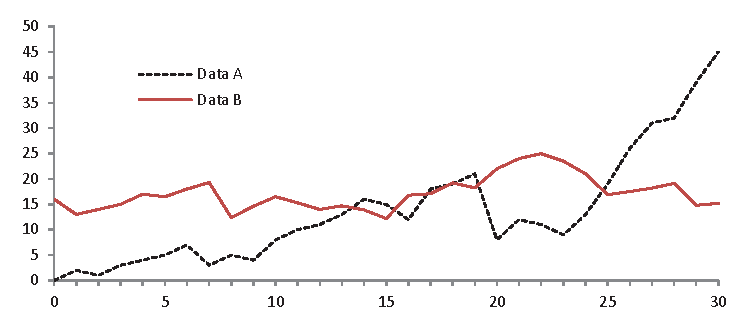
\includegraphics[width=\textwidth]{fig1.eps}
\caption{A figure caption is always placed below the illustration.
Please note that short captions are centered, while long ones are
justified by the macro package automatically.} \label{fig1}
\end{figure}

\begin{theorem}
This is a sample theorem. The run-in heading is set in bold, while
the following text appears in italics. Definitions, lemmas,
propositions, and corollaries are styled the same way.
\end{theorem}
%
% the environments 'definition', 'lemma', 'proposition', 'corollary',
% 'remark', and 'example' are defined in the LLNCS documentclass as well.
%
\begin{proof}
Proofs, examples, and remarks have the initial word in italics,
while the following text appears in normal font.
\end{proof}
For citations of references, we prefer the use of square brackets
and consecutive numbers. Citations using labels or the author/year
convention are also acceptable. The following bibliography provides
a sample reference list with entries for journal
articles~\cite{ref_article1}, an LNCS chapter~\cite{ref_lncs1}, a
book~\cite{ref_book1}, proceedings without editors~\cite{ref_proc1},
and a homepage~\cite{ref_url1}. Multiple citations are grouped
\cite{ref_article1,ref_lncs1,ref_book1},
\cite{ref_article1,ref_book1,ref_proc1,ref_url1}.

\begin{credits}
\subsubsection{\ackname} A bold run-in heading in small font size at the end of the paper is
used for general acknowledgments, for example: This study was funded
by X (grant number Y).

\subsubsection{\discintname}
It is now necessary to declare any competing interests or to specifically
state that the authors have no competing interests. Please place the
statement with a bold run-in heading in small font size beneath the
(optional) acknowledgments\footnote{If EquinOCS, our proceedings submission
system, is used, then the disclaimer can be provided directly in the system.},
for example: The authors have no competing interests to declare that are
relevant to the content of this article. Or: Author A has received research
grants from Company W. Author B has received a speaker honorarium from
Company X and owns stock in Company Y. Author C is a member of committee Z.
\end{credits}
%
% ---- Bibliography ----
%
% BibTeX users should specify bibliography style 'splncs04'.
% References will then be sorted and formatted in the correct style.
%
% \bibliographystyle{splncs04}
% \bibliography{mybibliography}
%
\begin{thebibliography}{8}
\bibitem{ref_article1}
Author, F.: Article title. Journal \textbf{2}(5), 99--110 (2016)

\bibitem{ref_lncs1}
Author, F., Author, S.: Title of a proceedings paper. In: Editor,
F., Editor, S. (eds.) CONFERENCE 2016, LNCS, vol. 9999, pp. 1--13.
Springer, Heidelberg (2016). \doi{10.10007/1234567890}

\bibitem{ref_book1}
Author, F., Author, S., Author, T.: Book title. 2nd edn. Publisher,
Location (1999)

\bibitem{ref_proc1}
Author, A.-B.: Contribution title. In: 9th International Proceedings
on Proceedings, pp. 1--2. Publisher, Location (2010)

\bibitem{ref_url1}
LNCS Homepage, \url{http://www.springer.com/lncs}, last accessed 2023/10/25
\end{thebibliography}
\end{document}
